\section{Introduction}

D'après Wikipedia \cite{Wiki}, \say{la \textit{bio-inspiration} est un changement de paradigme qui conduit des concepteurs à s'inspirer de la nature pour développer de nouveaux systèmes}. Il s'agit d'une branche de la robotique en plein essor et émergente, qui, dans certains cas, elle peut être considérée en opposition au concept de l'intelligence artificielle (IA), le paradigme qui s'inspire du cerveau humain pour développer des méthodes d'apprentissage mais qui est aujourd'hui assez limité pour être embarqué du point de vue technologique (autonomie, capacités de calcul, etc.). À partir de cela, la \textit{bio-inspiration} se réoriente vers une nouvelle approche qui essaie de reproduire la nature (mouvements ou comportements) pour repousser les limites de la technologie actuelle. En particulier, la \textit{bio-inspiration} consiste à s'inspirer des animaux pour doter de capacités d'autonomie aux robots, c'est-à-dire donner aux robots des capacités de perception, d'interprétation, de décision et d'action sur son environnement sans intervention externe. 

Dans ce rapport, nous aborderons une technologie bio-inspirée: la détection électrique, le sens électrique ou l'électrolocation. Cette approche vient des poissons électriques tels que les \textit{Gymnotiformes} ou les \textit{Mormyridés}, et d'après \cite{Panama}, \say{les décharges électriques chez ces animaux [...] sont utilisées pour la navigation, la détection et la capture de proies, principalement la nuit, ainsi que dans les eaux turbides}. De ce fait nous retrouvons deux modes de perception par le sens électrique: l'électrolocation active, que nous retrouvons chez des poissons qui génèrent des décharges électriques par des muscles spécialisés (myogénie) ou par des cellules nerveuses (neurogénie), ou passive, que nous retrouvons chez de poissons qui ne génèrent pas des décharges électriques mais par une source externe. En particulier, dans ce rapport, nous traiterons l'électrolocation active avec une simulation en Matlab. La Figure \ref{fig:poisson_champ}.(a) montre une photo du poisson-éléphant \textit{Gnathonemus petersii}, un poisson qui a une mauvaise vue, et utilise un champ électrique généré par des contractions musculaires pour trouver de la nourriture, se repérer dans l'obscurité ou la turbidité des eaux, et même trouver un partenaire, d'après \cite{Wiki2}. À côté, la Figure \ref{fig:poisson_champ}.(b) montre le champ électrique simulé autour du corps d'un poisson doté du sens électrique que je présente ici. 

\begin{figure}[h!]
    \centering
    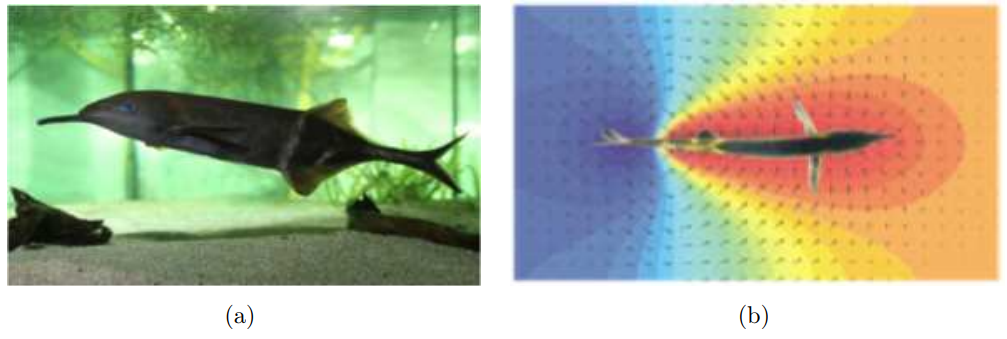
\includegraphics[width=0.9\textwidth]{doc/img/poisson_champ.png}
    \caption{\centering Photo du poisson \textit{Gnathonemus petersii} (a) et champ électrique autour du corps du poisson (b), image extraite de \cite{BENACHENHOU2014}.}
    \label{fig:poisson_champ}
\end{figure}

L'objectif de ce TP est de créer un simulateur pour la navigation 2D d'un poisson dans un aquarium, qui intègre une loi de contrôle pour l'évitement d'obstacles (peu importe si isolant ou conducteur) en cinématique. 
Ce rapport comprend 3 chapitres à la suite de cette introduction. Dans le premier chapitre, nous présenterons le robot poisson simulé, une résolution au problème d'électrolocation active dite \og méthode des réflexions \fg{} utilisée dans le simulateur, et les résultats obtenus pour des petits objets conducteurs et isolants. Le deuxième chapitre présente la démarche de commande utilisée pour simuler le mouvement d'un poisson en évitant les obstacles, puis les résultats obtenus pour cette loi de commande. 

